\needspace{10\baselineskip}
\chapter{Rilevamento delle differenze tra fotogrammi}
\label{cha:diff}

Una funzionalità innovativa introdotta dal sistema LODE è la possibilità per gli studenti di acquisire in tempo reale durante le lezioni degli screenshot di quanto viene proiettato. Dal punto di vista tecnico questo significa che il "box" deve poter acquisire singolarmente dei fotogrammi dall'ingresso HDMI e inviarli al server.

Per evitare che richieste di screenshot molto vicine provochino inutili upload di screenshot, è possibile implementare un sistema per rilevare se uno screenshot è effettivamente nuovo, e in caso negativo riusare quello precedente.

\section{Il formato YUV420SP}
\label{sec:diff_yuv}

Prima di iniziare a lavorare sul confronto delle immagini, è opportuno familiarizzare con il formato YUV420SP, che si incontra frequentemente nello sviluppo Android con il nome di NV12 o NV21.

Prima di tutto, YUV420 è un termine approssimativo per riferirsi a Y'CbCr 4:2:0, un formato di pixel appartenente alla famiglia Y'CbCr, in cui il colore di un pixel è scomposto nelle componenti Y' (luminanza, scala di grigi\footnotemark{}), Cb/U (proiezione del blu) e Cr/V (proiezione del rosso).\cite{yuv}

\footnotetext{La suddivisione delle componenti in Y, U e V deriva dal mondo analogico, quando c'era la necessità di supportare sia tv in bianco e nero che a colori. Avere una componente in scala di grigi isolata permette infatti di mantenere la retrocompatibilità pur introducendo il colore. In ambito digitale, è più corretto usare il termine Y'CbCr anziché YUV.}

Questa divisione permette di applicare una tecnica chiamata sottocampionamento della crominanza, che riduce la risoluzione delle due componenti della crominanza (Cb e Cr), lasciando a piena risoluzione la luminanza. Questa tecnica è fondata sul fatto che l'occhio umano è molto più sensibile all'intensità di luce che al colore (figura \ref{fig:diff_mit}), per cui anche se riduciamo i "bit" per la rappresentazione della crominanza la differenza è nella gran parte dei casi quasi impercettibile.\cite{luminance} La grandissima maggioranza dei video normalmente fruibili tramite Internet o la televisione digitale sono codificati con un formato dei pixel Y'CbCr 4:2:0, che è il più diffuso in ambiti non professionali.

% https://twitter.com/AkiyoshiKitaoka/status/1028473566193315841

\begin{figure}[htbp]
	\centering
	
	\begin{subfigure}[t]{0.45\textwidth}
		\centering
		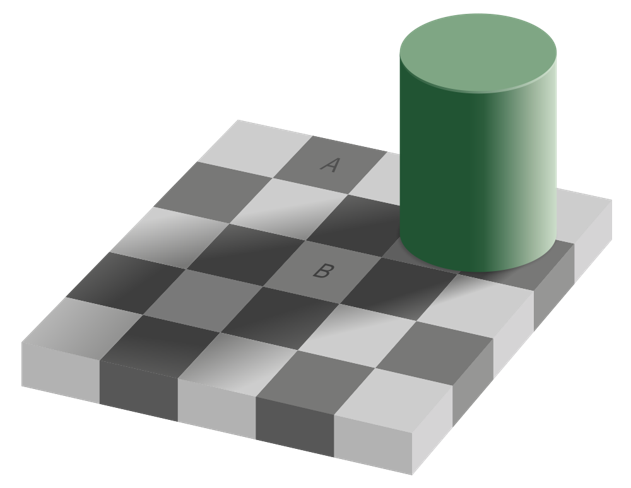
\includegraphics[width=\textwidth]{res/mit1.png}
	\end{subfigure}%
	~ 
	\begin{subfigure}[t]{0.45\textwidth}
		\centering
		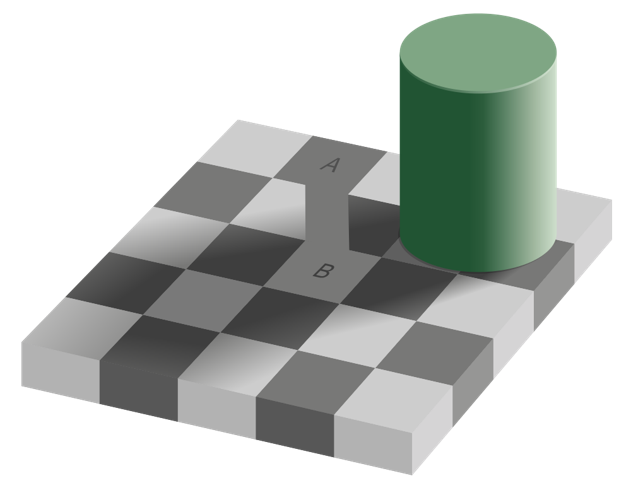
\includegraphics[width=\textwidth]{res/mit2.png}
	\end{subfigure}
	
	\caption{Rappresentazione grafica realizzata dal MIT\protect\footnotemark{} per mostrare come l'occhio umano è molto sensibile all'intensità della luce (luminanza). L'illusione ottica fa credere che i due riquadri A e B siano di una sfumatura di grigio diversa, quando in realtà sono identici.}
	\label{fig:diff_mit}
\end{figure}

\footnotetext{\url{http://persci.mit.edu/gallery/checkershadow}}

La figura \ref{fig:diff_yuv420} mostra il sottocampionamento della crominanza 4:2:0 applicato a una griglia di dimensione 4 x 2 pixel. La componente Y, cioè la luminanza, viene campionata a piena risoluzione, e cioè per ogni pixel vengono catturate informazioni piene. L'informazione sulla crominanza, composta dalla componente blu e rossa\footnotemark{}, viene invece catturata a $1/4$ della risoluzione, e cioè è condivisa tra 4 pixel. In confronto a RGB24, questo formato richiede in media 12 bit per pixel anziché 24 (da qui il nome "NV12"), con un risparmio di dati del 50\% senza sacrificare visibilmente la qualità complessiva.

\footnotetext{L'informazione sul verde non è esplicitamente memorizzata ma rappresenta circa il 60\% della componente Y: \url{https://news.ycombinator.com/item?id=1892248}}

\begin{figure}[htbp]
	\centering
	
	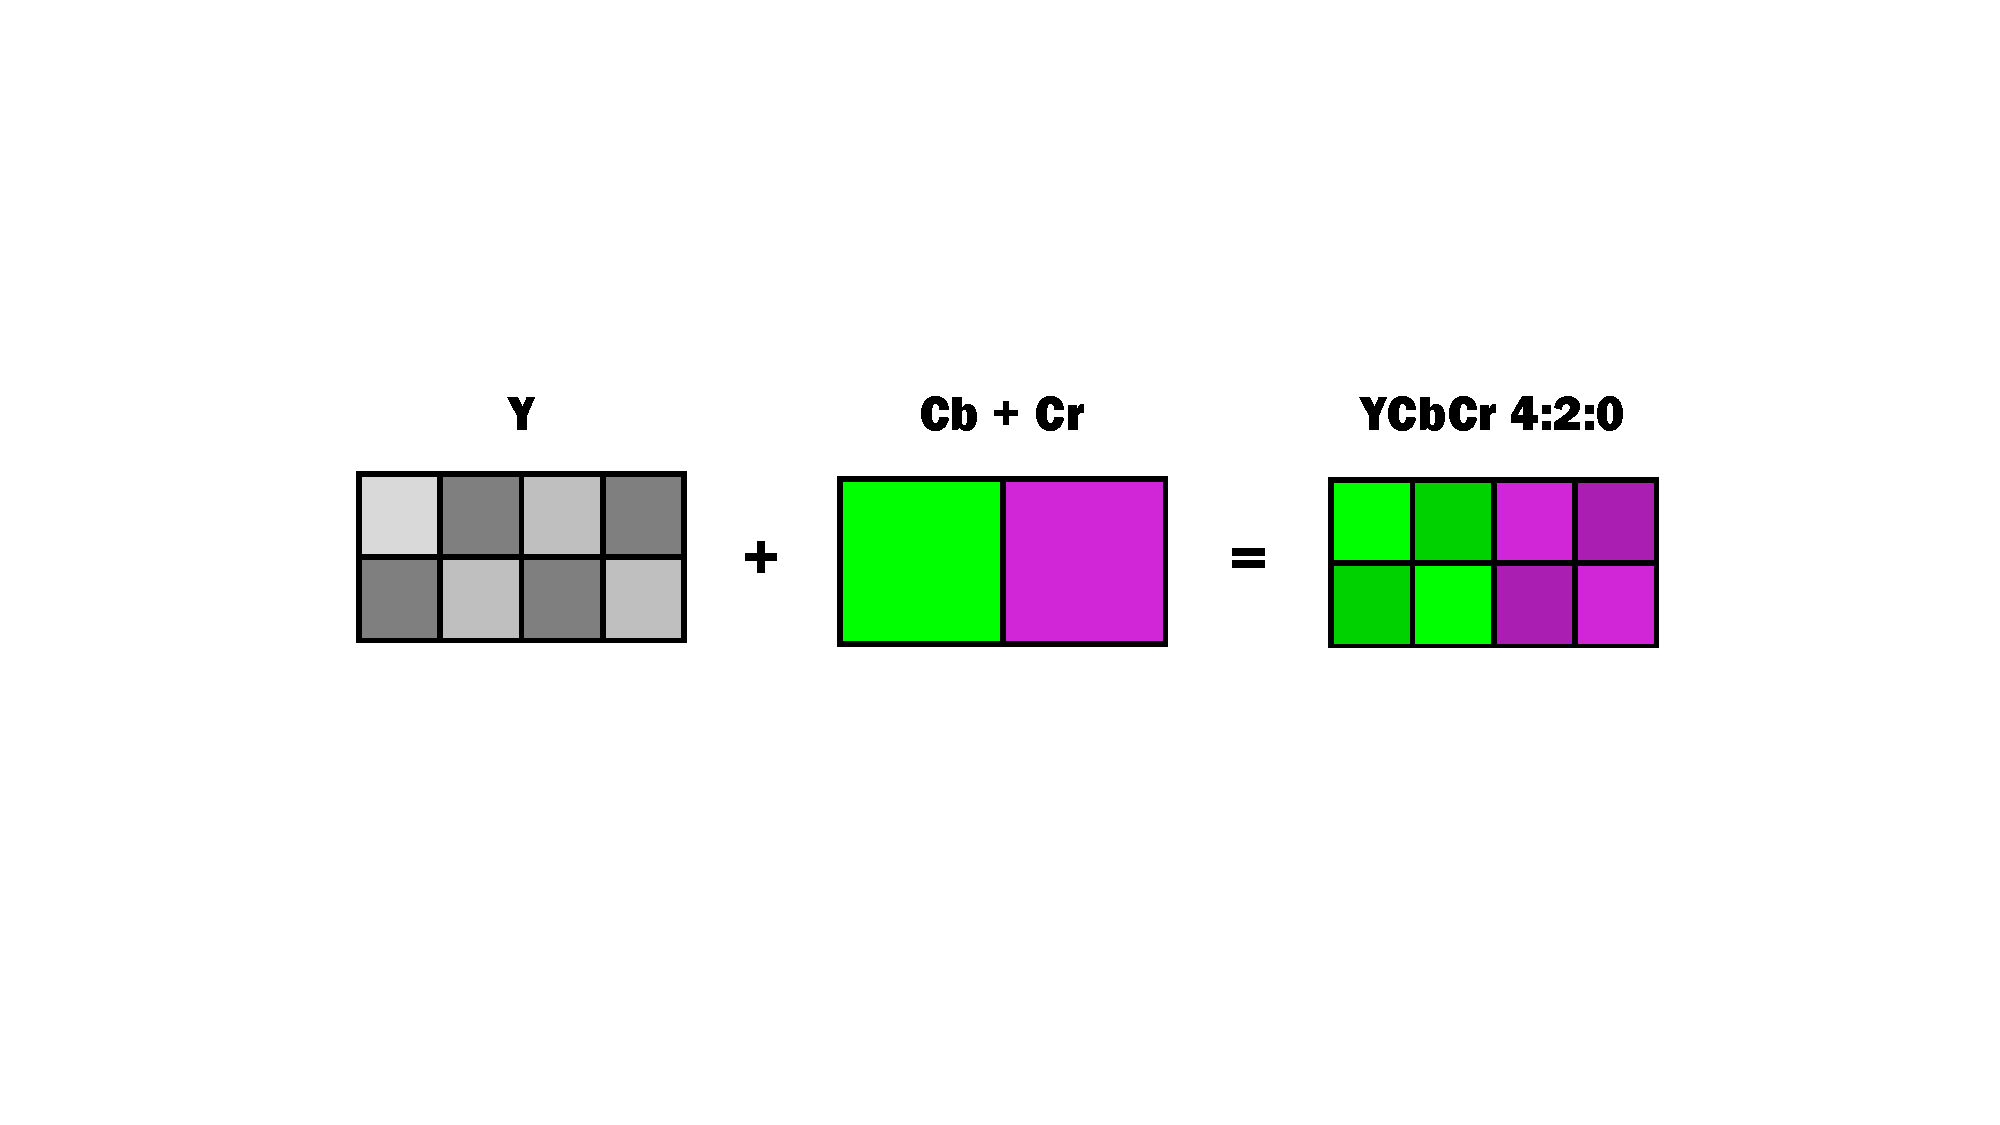
\includegraphics[width=0.8\textwidth]{res/yuv420.pdf}
%	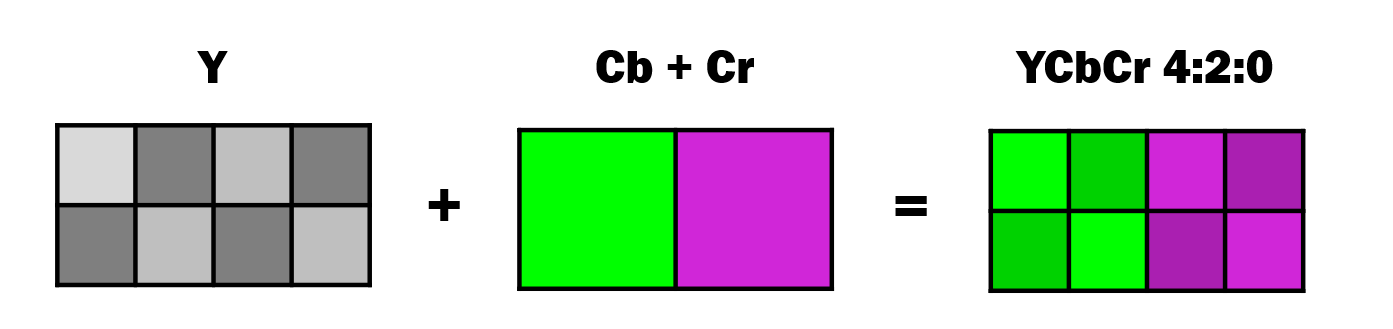
\includegraphics[width=0.9\textwidth]{res/yuv420.png}
	
	\caption{Sottocampionamento della crominanza 4:2:0. Il 4 indica la larghezza della griglia, che ha altezza 2 (fissa). Il 2 indica che la risoluzione orizzontale è dimezzata (2 campioni), mentre lo zero che non ci sono campioni diversi tra la prima e la seconda riga.}
	\label{fig:diff_yuv420}
\end{figure}

Nel momento in cui YUV420 deve essere rappresentato sotto forma di bit, i tre piani (Y, U e V) vengono isolati. Ad esempio, un pixel verrebbe rappresentato così (ogni lettera è un bit)\footnote{\url{https://wiki.videolan.org/YUV}}:

\definecolor{ChromaBlue}{HTML}{1160c6}
\definecolor{ChromaRed}{HTML}{E60000}
\definecolor{ChromaSP}{HTML}{ff9c00}

\tikzset{
	pixel/.style={node distance=1pt,font=\sffamily},
	pixelY/.style={pixel,fill=black!15},
	pixelU/.style={pixel,fill=ChromaBlue,text=white},
	pixelV/.style={pixel,fill=ChromaRed,text=white},
	pixelSP/.style={pixel,fill=ChromaSP,text=white},
}

\begin{figure}[H]
	\begin{tikzpicture}
	\node[pixelY] (y) {YYYYYYYY};
	\node[pixelU,right=of y] (u) {UU};
	\node[pixelV,right=of u] {VV};
	\end{tikzpicture}
\end{figure}

Mentre in RGB ciascun pixel richiederebbe 8 bit per canale, in YUV420 i due piani della crominanza (blu e rosso) ne richiedono solo $1/4$, cioè 2.

Di conseguenza, 2 pixel sarebbero rappresentati così, dove ciascuna coppia di U/V è relativa a un pixel:

\begin{figure}[H]
	\begin{tikzpicture}
	\node[pixelY] (y) {YYYYYYYY YYYYYYYY};
	\node[pixelU,right=of y] (u) {UU UU};
	\node[pixelV,right=of u] {VV VV};
	\end{tikzpicture}
\end{figure}

Il formato YUV420SP è invece una variante di YUV420 \emph{Semi Planar}, che significa che i piani U e V sono interlacciati in un unico piano. Un pixel YUV420SP (NV12) verrebbe quindi rappresentato così:

\begin{figure}[H]
	\begin{tikzpicture}
	\node[pixelY] (y) {YYYYYYYY};
	\node[pixelSP,right=of y] {UVUV};
	\end{tikzpicture}
\end{figure}

E 2 pixel così:

\begin{figure}[H]
	\begin{tikzpicture}
	\node[pixelY] (y) {YYYYYYYY YYYYYYYY};
	\node[pixelSP,right=of y] {UVUV UVUV};
	\end{tikzpicture}
\end{figure}

Come accennato, esiste anche il formato NV21, supportato da Android, che è uguale a NV12 ma con la differenza che le componenti U e V all'interno del secondo piano sono scambiate, come mostrato nell'esempio:

\begin{figure}[H]
	\begin{tikzpicture}
	\node[pixelY] (y) {YYYYYYYY YYYYYYYY};
	\node[pixelSP,right=of y] {VUVU VUVU};
	\end{tikzpicture}
\end{figure}

Come si nota dagli schemi, in NV12/NV21 le informazioni sulla luminanza sono raggruppate all'inizio e utilizzano 1 byte per pixel. Questa caratteristica tornerà utile nelle prossime sezioni, in combinazione al fatto che Android fornisce le immagini acquisite dall'ingresso HDMI anche in formato NV21.

\section{Confronto pixel per pixel}
\label{sec:diff_full}

La prima possibilità esplorata è la più immediata: catturare i fotogrammi in formato "non compresso" (NV21) e confrontarli byte per byte. La prima coppia di byte che ha valori diversi determina l'esistenza di una differenza tra i due fotogrammi.

Ricordando la classe \texttt{Camera} di Android introdotta nella sezione \ref{sec:hdmi_camera1}, si può sfruttare il metodo \texttt{setPreviewCallback(...)} per ricevere i dati "raw" che vengono mostrati su schermo.\footnote{\url{https://developer.android.com/reference/android/hardware/Camera.PreviewCallback.html}}

\begin{minted}{java}
camera.setPreviewCallback(new PreviewCallback() {
    @Override
    public void onPreviewFrame(byte[] data, Camera camera) {
        // `data` contiene i dati in formato NV21
    }
});
\end{minted}

Supponendo ora di avere due array di byte contenenti due fotogrammi catturati in momenti diversi, si può concludere che se le due immagini sono identiche anche i valori dei pixel e quindi i relativi "byte" saranno identici. Di conseguenza, per confrontare i due array si può usare il metodo \texttt{Arrays.equals(arr1, arr2)} contenuto in \texttt{java.util}, che è implementato con un ciclo che confronta gli array byte per byte e si ferma eventualmente alla prima differenza.\footnote{\url{https://hg.openjdk.java.net/jdk8/jdk8/jdk/file/687fd7c7986d/src/share/classes/java/util/Arrays.java\#l2668}}

Questo metodo di rilevamento delle differenze è stato verificato e funziona in modo affidabile, ma ha lo svantaggio non trascurabile di non essere molto performante. Su uno degli hardware testati, il confronto di due fotogrammi con risoluzione 1920 x 1080 (e quindi di $3\,110\,400$ byte\footnote{$(1920 \cdot 1080) / 2$}) richiedeva circa 400 millisecondi.

Come accennato nella sezione \ref{sec:diff_yuv}, l'occhio umano è più sensibile alla luminanza che alla crominanza. Si può quindi tentare di ridurre la quantità di byte da confrontare selezionando soltanto il piano Y, che rappresenta la luminanza.

In questo caso il confronto va implementato manualmente per considerare soltanto una parte dell'array, quella corrispondente al primo piano, che qua si suppone utilizzi un byte per pixel come nel caso di NV12/NV21:

\begin{minted}{java}
public boolean isLuminanceEqual(byte[] arr1, byte[] arr2, int width, int height) {
    int maxLength = width * height;
    
    for (int i = 0; i < maxLength; i++) {
        if (arr1[i] != arr2[i]) {
            return false;
        }
    }
    
    return true;
}
\end{minted}

Assumendo una risoluzione di 1920 x 1080 pixel, il numero di byte da verificare si riduce a $2\,073\,600$, cioè $2/3$ del totale. La riduzione è interessante ma non risolutiva in termini di prestazioni.

\section{Confronto parziale}
\label{sec:diff_parziale}

Una soluzione alternativa a confrontare l'intera immagine è individuare un sottoinsieme di pixel, distribuito in modo da rendere sufficientemente probabile il rilevamento delle differenze.

Si parte dal presupposto che durante una lezione vengano proiettati contenuti le cui variazioni sono abbastanza evidenti. Si pensi ad esempio a una presentazione di slide dove con il passaggio da una pagina all'altra varia l'intero contenuto proiettato o viene aggiunta una riga di testo, oppure a una finestra del browser dove lo scorrimento della pagina provoca lo spostamento di tutto il contenuto.

Si può quindi costruire una griglia virtuale i cui punti di intersezione rappresentano i pixel da confrontare, come mostrato in figura \ref{fig:diff_slide1}. L'approccio funziona bene in molti casi: prendendo come riferimento la figura si immagini come l'aggiunta di una riga verrebbe facilmente rilevata dai punti stabiliti (che sono fissi).

\tikzset{
	gridline/.style={line width=0.4pt,color=lightgray},
	gridarrow/.style={-{Straight Barb},very thick,red},
}

\begin{figure}[htbp]
	\centering

	\begin{tikzpicture}
	% https://tex.stackexchange.com/questions/9559/drawing-on-an-image-with-tikz

	\node[anchor=south west,inner sep=0] (image) at (0,0)
		{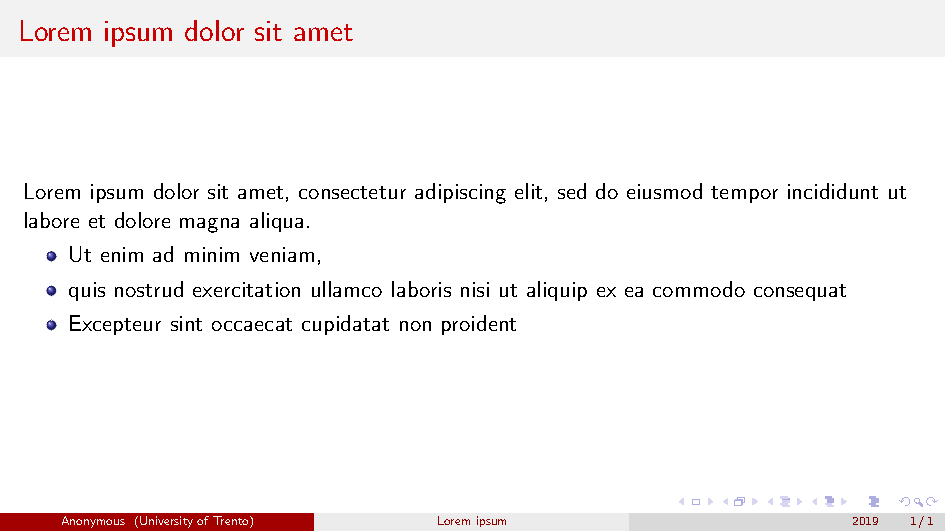
\includegraphics[width=0.9\textwidth]{res/test-slide/beamer.pdf}};
	
	\begin{scope}[x={(image.south east)},y={(image.north west)}]
%	\draw[color=black,thick,xstep=.1,ystep=.1] (0,0) grid (1,1);
	\foreach \x in {1,...,9} { \draw[gridline] (\x/10,0) -- (\x/10,1); }
	\foreach \y in {1,...,49} { \draw[gridline] (0,\y/50) -- (1,\y/50); }
	\end{scope}
	
	\end{tikzpicture}
	
	\caption{La griglia è composta da 9 righe orizzontali e 49 verticali, per un totale di 441 punti.}
	\label{fig:diff_slide1}
\end{figure}

Ci sono tuttavia altri casi in cui i cambiamenti potrebbero riguardare delle aree non rilevate dai punti selezionati, come si deduce dalla figura \ref{fig:diff_slide2}.

\begin{figure}[htbp]
	\centering
	
	\begin{subfigure}[t]{0.5\textwidth}
		\begin{tikzpicture}
		\node[anchor=south west,inner sep=0] (image) at (0,0)
		{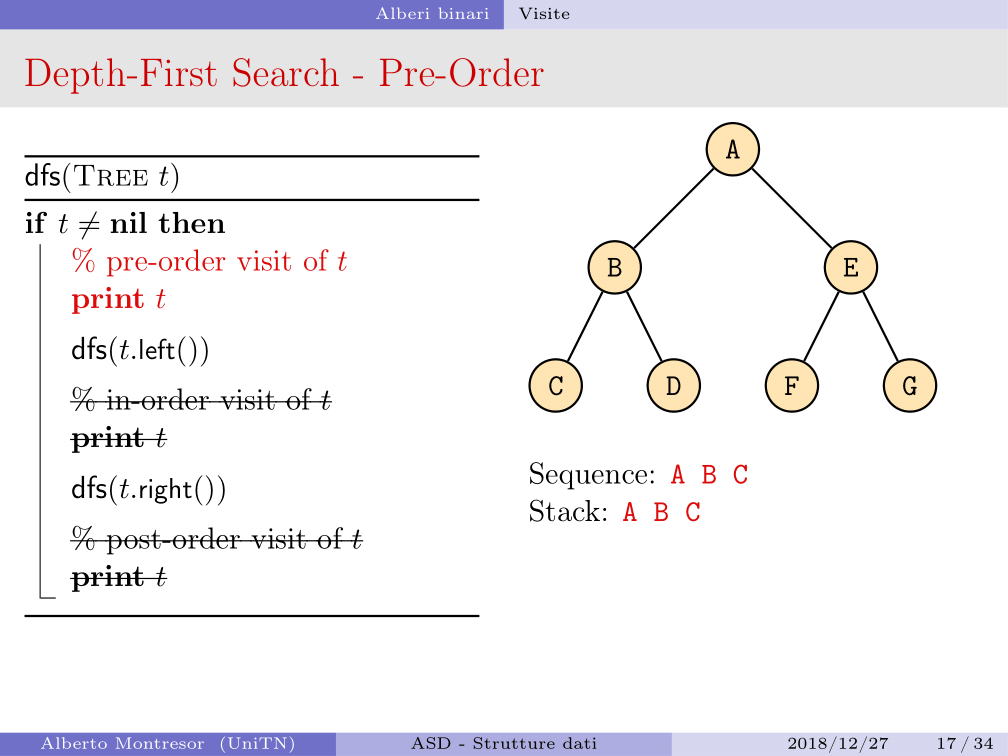
\includegraphics[width=\textwidth]{res/slide3.png}};
		
		\begin{scope}[x={(image.south east)},y={(image.north west)}]
		\foreach \x in {1,...,9} { \draw[gridline] (\x/10,0) -- (\x/10,1); }
		\foreach \y in {1,...,49} { \draw[gridline] (0,\y/50) -- (1,\y/50); }
		
		\draw[gridarrow] (0.62,0.15) -- (0.68,0.29);
		\end{scope}
		
		\end{tikzpicture}
	\end{subfigure}%
	~ 
	\begin{subfigure}[t]{0.5\textwidth}
		\begin{tikzpicture}
		\node[anchor=south west,inner sep=0] (image) at (0,0)
		{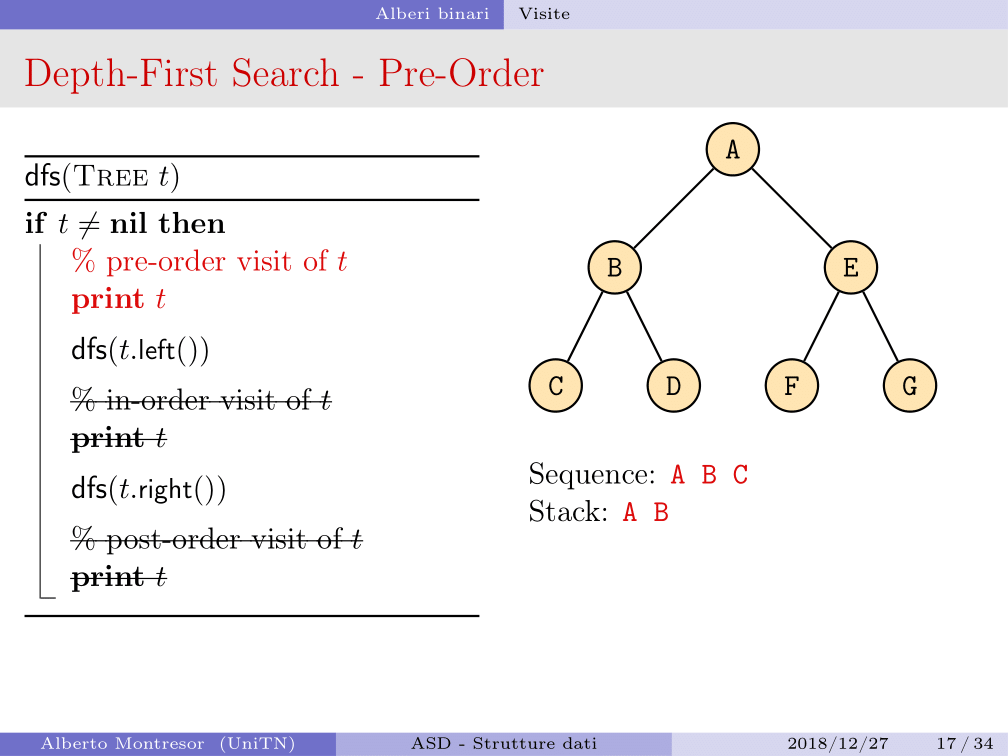
\includegraphics[width=\textwidth]{res/slide4.png}};
		
		\begin{scope}[x={(image.south east)},y={(image.north west)}]
		\foreach \x in {1,...,9} { \draw[gridline] (\x/10,0) -- (\x/10,1); }
		\foreach \y in {1,...,49} { \draw[gridline] (0,\y/50) -- (1,\y/50); }
		
		\draw[gridarrow] (0.62,0.15) -- (0.68,0.29);
		\end{scope}
		
		\end{tikzpicture}
	\end{subfigure}
	
	\caption{Anche in questo caso i punti di intersezione sono 441. Si noti però che l'area puntata dalla freccia presenta delle differenze tra i due fotogrammi che non vengono rilevate. Le immagini sono state gentilmente offerte dal prof. Alberto Montresor.}
	\label{fig:diff_slide2}
\end{figure}

Si possono quindi considerare delle strategie alternative che permettono di aggirare questo problema. Ad esempio:

\begin{itemize}
	\item il numero di righe e colonne della griglia può essere ricalcolato ad ogni controllo aggiungendo un fattore di casualità. Se un controllo non riesce a rilevare differenze, la volta successiva potrebbe invece riuscirci, dato che i pixel campione saranno diversi (con ragionevole sicurezza);
	\item la distanza orizzontale e verticale tra i punti può essere mantenuta costante, ma si può invece aggiungere uno scorrimento graduale verso destra e verso il basso dei punti, in modo da coprire aree diverse ad ogni controllo;
	\item la strategia di scegliere un numero casuale di righe e colonne può essere resa più intelligente, per evitare che la stessa coordinata orizzontale e/o verticale venga considerata in diverse combinazioni della griglia.
\end{itemize}

La strategia del primo punto è stata sperimentata su diversi contenuti e ha dato ottimi risultati. Gran parte dei cambiamenti venivano rilevati al primo controllo, e in ogni caso entro 3-4 controlli. Nei test l'intervallo di verifica delle differenze era 500 millisecondi, per cui il ritardo massimo di rilevamento risultava di circa 2 secondi.

Nei test effettuati il numero di colonne e righe della griglia veniva scelto in modo casuale ad ogni controllo, scegliendo rispettivamente dall'intervallo $[10, 20]$ e $[60, 80]$. Con questi dati, nel peggiore dei casi il numero di pixel/byte da verificare è $1\,600$, un valore estremamente limitato se confrontato con i 3 milioni di byte della sezione \ref{sec:diff_full}. Le prestazioni di questa soluzione sono risultate di conseguenza molto buone, con un tempo di confronto limitato a pochi millisecondi. \hl{da ri-verificare con precisione}

\hl{long polling?}

\section{Estrazione slide in post-produzione}
\label{sec:diff_postprod}

Lorem ipsum dolor sit amet.

